
\documentclass[10pt,conference]{IEEEtran}


% Some very useful LaTeX packages include:
% (uncomment the ones you want to load)


% *** MISC UTILITY PACKAGES ***
%
%\usepackage{ifpdf}
% Heiko Oberdiek's ifpdf.sty is very useful if you need conditional
% compilation based on whether the output is pdf or dvi.
% usage:
% \ifpdf
%   % pdf code
% \else
%   % dvi code
% \fi
% The latest version of ifpdf.sty can be obtained from:
% http://www.ctan.org/pkg/ifpdf
% Also, note that IEEEtran.cls V1.7 and later provides a builtin
% \ifCLASSINFOpdf conditional that works the same way.
% When switching from latex to pdflatex and vice-versa, the compiler may
% have to be run twice to clear warning/error messages.




\usepackage{hyperref}


% *** CITATION PACKAGES ***
%
\usepackage{cite}
% cite.sty was written by Donald Arseneau
% V1.6 and later of IEEEtran pre-defines the format of the cite.sty package
% \cite{} output to follow that of the IEEE. Loading the cite package will
% result in citation numbers being automatically sorted and properly
% "compressed/ranged". e.g., [1], [9], [2], [7], [5], [6] without using
% cite.sty will become [1], [2], [5]--[7], [9] using cite.sty. cite.sty's
% \cite will automatically add leading space, if needed. Use cite.sty's
% noadjust option (cite.sty V3.8 and later) if you want to turn this off
% such as if a citation ever needs to be enclosed in parenthesis.
% cite.sty is already installed on most LaTeX systems. Be sure and use
% version 5.0 (2009-03-20) and later if using hyperref.sty.
% The latest version can be obtained at:
% http://www.ctan.org/pkg/cite
% The documentation is contained in the cite.sty file itself.






% *** GRAPHICS RELATED PACKAGES ***
%
\ifCLASSINFOpdf
   \usepackage[pdftex]{graphicx}
  % declare the path(s) where your graphic files are
   \graphicspath{{figs/}}
  % and their extensions so you won't have to specify these with
  % every instance of \includegraphics
   \DeclareGraphicsExtensions{.pdf,.jpeg,.png}
\else
  % or other class option (dvipsone, dvipdf, if not using dvips). graphicx
  % will default to the driver specified in the system graphics.cfg if no
  % driver is specified.
   \usepackage[dvips]{graphicx}
  % declare the path(s) where your graphic files are
   \graphicspath{{../figs/}}
  % and their extensions so you won't have to specify these with
  % every instance of \includegraphics
   \DeclareGraphicsExtensions{.eps}
\fi
% graphicx was written by David Carlisle and Sebastian Rahtz. It is
% required if you want graphics, photos, etc. graphicx.sty is already
% installed on most LaTeX systems. The latest version and documentation
% can be obtained at: 
% http://www.ctan.org/pkg/graphicx
% Another good source of documentation is "Using Imported Graphics in
% LaTeX2e" by Keith Reckdahl which can be found at:
% http://www.ctan.org/pkg/epslatex
%
% latex, and pdflatex in dvi mode, support graphics in encapsulated
% postscript (.eps) format. pdflatex in pdf mode supports graphics
% in .pdf, .jpeg, .png and .mps (metapost) formats. Users should ensure
% that all non-photo figures use a vector format (.eps, .pdf, .mps) and
% not a bitmapped formats (.jpeg, .png). The IEEE frowns on bitmapped formats
% which can result in "jaggedy"/blurry rendering of lines and letters as
% well as large increases in file sizes.
%
% You can find documentation about the pdfTeX application at:
% http://www.tug.org/applications/pdftex





% *** MATH PACKAGES ***
%
\usepackage[cmex10]{amsmath}
% A popular package from the American Mathematical Society that provides
% many useful and powerful commands for dealing with mathematics.
%
% Note that the amsmath package sets \interdisplaylinepenalty to 10000
% thus preventing page breaks from occurring within multiline equations. Use:
\interdisplaylinepenalty=2500
% after loading amsmath to restore such page breaks as IEEEtran.cls normally
% does. amsmath.sty is already installed on most LaTeX systems. The latest
% version and documentation can be obtained at:
% http://www.ctan.org/pkg/amsmath
\usepackage{amsthm}
\newtheorem{definition}{Definition}




% *** SPECIALIZED LIST PACKAGES ***
%
\usepackage{algorithmic}
% algorithmic.sty was written by Peter Williams and Rogerio Brito.
% This package provides an algorithmic environment fo describing algorithms.
% You can use the algorithmic environment in-text or within a figure
% environment to provide for a floating algorithm. Do NOT use the algorithm
% floating environment provided by algorithm.sty (by the same authors) or
% algorithm2e.sty (by Christophe Fiorio) as the IEEE does not use dedicated
% algorithm float types and packages that provide these will not provide
% correct IEEE style captions. The latest version and documentation of
% algorithmic.sty can be obtained at:
% http://www.ctan.org/pkg/algorithms
% Also of interest may be the (relatively newer and more customizable)
% algorithmicx.sty package by Szasz Janos:
% http://www.ctan.org/pkg/algorithmicx




% *** ALIGNMENT PACKAGES ***
%
\usepackage{array}
% Frank Mittelbach's and David Carlisle's array.sty patches and improves
% the standard LaTeX2e array and tabular environments to provide better
% appearance and additional user controls. As the default LaTeX2e table
% generation code is lacking to the point of almost being broken with
% respect to the quality of the end results, all users are strongly
% advised to use an enhanced (at the very least that provided by array.sty)
% set of table tools. array.sty is already installed on most systems. The
% latest version and documentation can be obtained at:
% http://www.ctan.org/pkg/array


% IEEEtran contains the IEEEeqnarray family of commands that can be used to
% generate multiline equations as well as matrices, tables, etc., of high
% quality.




% *** SUBFIGURE PACKAGES ***
\ifCLASSOPTIONcompsoc
  \usepackage[caption=false,font=normalsize,labelfont=sf,textfont=sf]{subfig}
\else
  \usepackage[caption=false,font=footnotesize]{subfig}
\fi
% subfig.sty, written by Steven Douglas Cochran, is the modern replacement
% for subfigure.sty, the latter of which is no longer maintained and is
% incompatible with some LaTeX packages including fixltx2e. However,
% subfig.sty requires and automatically loads Axel Sommerfeldt's caption.sty
% which will override IEEEtran.cls' handling of captions and this will result
% in non-IEEE style figure/table captions. To prevent this problem, be sure
% and invoke subfig.sty's "caption=false" package option (available since
% subfig.sty version 1.3, 2005/06/28) as this is will preserve IEEEtran.cls
% handling of captions.
% Note that the Computer Society format requires a larger sans serif font
% than the serif footnote size font used in traditional IEEE formatting
% and thus the need to invoke different subfig.sty package options depending
% on whether compsoc mode has been enabled.
%
% The latest version and documentation of subfig.sty can be obtained at:
% http://www.ctan.org/pkg/subfig




% *** FLOAT PACKAGES ***
%
%\usepackage{fixltx2e}
% fixltx2e, the successor to the earlier fix2col.sty, was written by
% Frank Mittelbach and David Carlisle. This package corrects a few problems
% in the LaTeX2e kernel, the most notable of which is that in current
% LaTeX2e releases, the ordering of single and double column floats is not
% guaranteed to be preserved. Thus, an unpatched LaTeX2e can allow a
% single column figure to be placed prior to an earlier double column
% figure.
% Be aware that LaTeX2e kernels dated 2015 and later have fixltx2e.sty's
% corrections already built into the system in which case a warning will
% be issued if an attempt is made to load fixltx2e.sty as it is no longer
% needed.
% The latest version and documentation can be found at:
% http://www.ctan.org/pkg/fixltx2e


%\usepackage{stfloats}
% stfloats.sty was written by Sigitas Tolusis. This package gives LaTeX2e
% the ability to do double column floats at the bottom of the page as well
% as the top. (e.g., "\begin{figure*}[!b]" is not normally possible in
% LaTeX2e). It also provides a command:
%\fnbelowfloat
% to enable the placement of footnotes below bottom floats (the standard
% LaTeX2e kernel puts them above bottom floats). This is an invasive package
% which rewrites many portions of the LaTeX2e float routines. It may not work
% with other packages that modify the LaTeX2e float routines. The latest
% version and documentation can be obtained at:
% http://www.ctan.org/pkg/stfloats
% Do not use the stfloats baselinefloat ability as the IEEE does not allow
% \baselineskip to stretch. Authors submitting work to the IEEE should note
% that the IEEE rarely uses double column equations and that authors should try
% to avoid such use. Do not be tempted to use the cuted.sty or midfloat.sty
% packages (also by Sigitas Tolusis) as the IEEE does not format its papers in
% such ways.
% Do not attempt to use stfloats with fixltx2e as they are incompatible.
% Instead, use Morten Hogholm'a dblfloatfix which combines the features
% of both fixltx2e and stfloats:
%
% \usepackage{dblfloatfix}
% The latest version can be found at:
% http://www.ctan.org/pkg/dblfloatfix




% *** PDF, URL AND HYPERLINK PACKAGES ***
%
\usepackage{url}
% url.sty was written by Donald Arseneau. It provides better support for
% handling and breaking URLs. url.sty is already installed on most LaTeX
% systems. The latest version and documentation can be obtained at:
% http://www.ctan.org/pkg/url
% Basically, \url{my_url_here}.




% *** Do not adjust lengths that control margins, column widths, etc. ***
% *** Do not use packages that alter fonts (such as pslatex).         ***
% There should be no need to do such things with IEEEtran.cls V1.6 and later.
% (Unless specifically asked to do so by the journal or conference you plan
% to submit to, of course. )


% correct bad hyphenation here
\hyphenation{op-tical net-works semi-conduc-tor}

%------------------------------------------------------------------------- 
% change the % on next lines to produce the final camera-ready version 
\newif\iffinal
\finalfalse
% \finaltrue
\newcommand{\cmtid}{99999}
%------------------------------------------------------------------------- 

\iffinal
\else
\usepackage[switch]{lineno}
\fi

\begin{document}
%
% paper title
% Titles are generally capitalized except for words such as a, an, and, as,
% at, but, by, for, in, nor, of, on, or, the, to and up, which are usually
% not capitalized unless they are the first or last word of the title.
% Linebreaks \\ can be used within to get better formatting as desired.
% Do not put math or special symbols in the title.
\title{Speeding Up PPO Training for Pokémon Red}


% author names and affiliations
% use a multiple column layout for up to two different
% affiliations

\iffinal

% author names and affiliations
% use a multiple column layout for up to three different
% affiliations
% \author{\IEEEauthorblockN{Caio Valente\\github.com/valentecaio\\12th June 2024}}

% conference papers do not typically use \thanks and this command
% is locked out in conference mode. If really needed, such as for
% the acknowledgment of grants, issue a \IEEEoverridecommandlockouts
% after \documentclass

% for over three affiliations, or if they all won't fit within the width
% of the page, use this alternative format:
% 
%\author{\IEEEauthorblockN{Michael Shell\IEEEauthorrefmark{1},
%Homer Simpson\IEEEauthorrefmark{2},
%James Kirk\IEEEauthorrefmark{3}, 
%Montgomery Scott\IEEEauthorrefmark{3} and
%Eldon Tyrell\IEEEauthorrefmark{4}}
%\IEEEauthorblockA{\IEEEauthorrefmark{1}School of Electrical and Computer Engineering\\
%Georgia Institute of Technology,
%Atlanta, Georgia 30332--0250\\ Email: see http://www.michaelshell.org/contact.html}
%\IEEEauthorblockA{\IEEEauthorrefmark{2}Twentieth Century Fox, Springfield, USA\\
%Email: homer@thesimpsons.com}
%\IEEEauthorblockA{\IEEEauthorrefmark{3}Starfleet Academy, San Francisco, California 96678-2391\\
%Telephone: (800) 555--1212, Fax: (888) 555--1212}
%\IEEEauthorblockA{\IEEEauthorrefmark{4}Tyrell Inc., 123 Replicant Street, Los Angeles, California 90210--4321}}

\else
  % \author{Caio Valente}
  \author{\IEEEauthorblockN{Caio Valente\\\href{https://github.com/valentecaio}{github.com/valentecaio}\\12th June 2024}}
  \linenumbers
\fi


% make the title area
\maketitle

% As a general rule, do not put math, special symbols or citations
% in the abstract
% \begin{abstract}
% The abstract goes here.
% \end{abstract}

% no keywords




% For peerreview papers, this IEEEtran command inserts a page break and
% creates the second title. It will be ignored for other modes.
\IEEEpeerreviewmaketitle



\section{Introduction}

In recent years, deep learning has made significant advances in various domains, including natural language processing, computer vision, and reinforcement learning. One fascinating application of reinforcement learning is training agents to play video games, which presents a complex and dynamic environment for learning. This paper focuses on training an agent to play Pokémon Red using the Proximal Policy Optimization (PPO) algorithm, with modifications to improve convergence speed and performance.

The original implementation from Peter Whidden \cite{ref:whidden} leveraged the PyBoy emulator API within a Gym environment, employing a Convolutional Neural Network (CNN) policy optimized using the Adam optimizer. The input to the network was based on the rendered images from the game. The primary objective was to maximize a reward function incorporating various game parameters, such as the number of frames visited, the total level of Pokémon in the party, and the frequency of healing events. Despite the promising framework and impressive results, the training process was notably slow, hindered by CPU-bound computations, the lengthy nature of game episodes and the slow convergence of the algorithm.

To address these challenges, this research explores several modifications to accelerate convergence, including dynamic learning rates, varying batch sizes, and incorporating weight decay using AdamW. Among the tested approaches, a constant large batch size with a constant learning rate proved most effective, reducing  substantially the necessary training time. However, this configuration resulted in the agent falling into a local minimum, prioritizing exploration and combat over capturing new Pokémon.




\section{Related Work}
The application of deep reinforcement learning (DRL) to video game environments has gained considerable attention, with notable successes in playing Atari games and other complex benchmarks. One of the pioneering works in this field is the Deep Q-Network (DQN) algorithm, introduced by Mnih et al. (2015) \cite{ref:dqn} and implemented by Roderick et al. (2017) \cite{ref:dqn2}, which demonstrated the capability of DRL agents to surpass human-level performance in various Atari 2600 games \cite{ref:ale}. DQN utilizes a convolutional neural network to approximate the Q-value function, enabling the agent to learn optimal policies directly from raw pixel inputs.

Subsequent advancements have built upon the DQN framework, addressing limitations such as instability and slow convergence. Proximal Policy Optimization (PPO), proposed by Schulman et al. (2017) \cite{ref:ppo}, has emerged as a robust alternative, combining the benefits of trust region policy optimization and importance sampling to achieve stable and efficient training. PPO has been successfully applied to a wide range of tasks, including robotic control, autonomous driving, and game playing. The PPO algorithm uses a policy gradient approach to optimize the policy and value functions. It maintains stability and efficiency by clipping the probability ratios during updates to ensure the new policies do not deviate excessively from the old ones. 

While significant progress has been made in mastering simpler games like Atari, more complex games such as Pokémon Red, an RPG game, still require further exploration. These games present a greater challenge due to their non-repetitive gameplay. The agent must navigate a narrative, handle recurrent events with straightforward dynamics like battles, and explore the map to advance the plot of the game. This complexity requires sophisticated learning strategies capable of dealing with both the game's strategic and exploratory aspects.

More recently, Peter Whidden proposed a PPO trained agent capable of beating the first gymnasium of Pokemon Red \cite{ref:whidden}. His original algorithm focuses on training an agent to play Pokémon Red using the algorithm within a custom Gym \cite{ref:gymnasium} environment. The primary objective is to maximize the agent's performance by rewarding various in-game achievements and penalizing setbacks, facilitating the agent's ability to explore, battle, and progress through the game effectively. The PPO model should maximize the total reward of the player for any action in any given state.

Whidden released his training code and a pretrained agent obtained through 439 million training steps, establishing it as the current state-of-the-art for this particular game. This extensive training process allowed the agent to develop strategies for exploring the game world, engaging in battles, and advancing through the storyline. However, the agent is not optimal - while it can successfully navigate up to and pass the first gym, it encounters difficulties and often gets stuck beyond that point. This limitation highlights the ongoing challenges and potential areas for improvement in developing reinforcement learning agents for complex RPG games like Pokémon Red.



\newpage



\section{Proposed Technique}

The pretrained model provided by the original author was trained for 439M steps, which would take approximately six days to run. However, it was trained running 128 episodes in parallel, on a machine with 128 cores and enough RAM to accommodate such a large rollout buffer size, likely leading to faster convergence and better generalization than what could be achieved on my 12 cores laptop. This means that achieving similar results on my machine could take up to 60 days.

Instead, my goal was to develop a model that could converge faster, within one day, achieving average results compared to the original setup. 

To achieve such, I used the same base algorithm as Whidden and experimented with the following hyperparameters: batch size, learning rate, entropy coefficient and weight decay.

The batch size refers to the number of training examples used in one iteration to update the model's parameters. A larger batch size typically provides a more stable estimate of the gradient, leading to smoother and potentially faster convergence, but requires more memory and computational resources. A smaller batch size may introduce more noise into the gradient estimation, which can sometimes help the model escape local minima but often results in less stable training.

The original implementation used the stable\_baselines3 library \cite{ref:stable-baselines3}, which lacked support for non-constant batch sizes. This work extended this library to include dynamic batch sizing and applied it in my experiments. The maximum batch size I was able to test was limited by my GPU memory (RTX 4050, 6G).

The learning rate determines the step size at each iteration while moving towards a minimum of the loss function. A higher learning rate allows the model to converge faster but risks overshooting the minimum, leading to divergence or oscillation. A lower learning rate provides more precise adjustments to the model parameters, which can result in more stable convergence but at the cost of longer training times. Dynamic learning rates adjust over time to balance these trade-offs, often starting high to speed up initial training and decreasing to refine the model's performance.

The entropy coefficient controls the entropy bonus added to the reward function, encouraging exploration by preventing the policy from becoming too deterministic too quickly. A higher entropy coefficient promotes more exploratory actions, helping the agent to discover potentially better strategies by exploring a broader range of actions. However, excessive exploration can slow down the convergence to an optimal policy. A lower entropy coefficient reduces exploration, allowing the model to exploit known good actions but risking premature convergence to suboptimal policies.

The weight decay is a hyperparameter of the AdamW optimizer. It is a regularization technique that helps prevent overfitting by penalizing large weights. This penalty term is added to the loss function, encouraging the model to keep the weights smaller and more generalized. In contrast to traditional L2 regularization, which directly modifies the gradients, AdamW decouples weight decay from the gradient updates, leading to more effective regularization. Applying weight decay can improve generalization by preventing the model from fitting noise in the training data. However, if set too high, it may hinder the model's ability to learn complex patterns in the data, resulting in underfitting.

In this work, I tried six variations of hyperparameters in the original PPO algorithm and compared their performance to the original retrained model.



\begin{figure*}[h]
  \centering
  \fbox{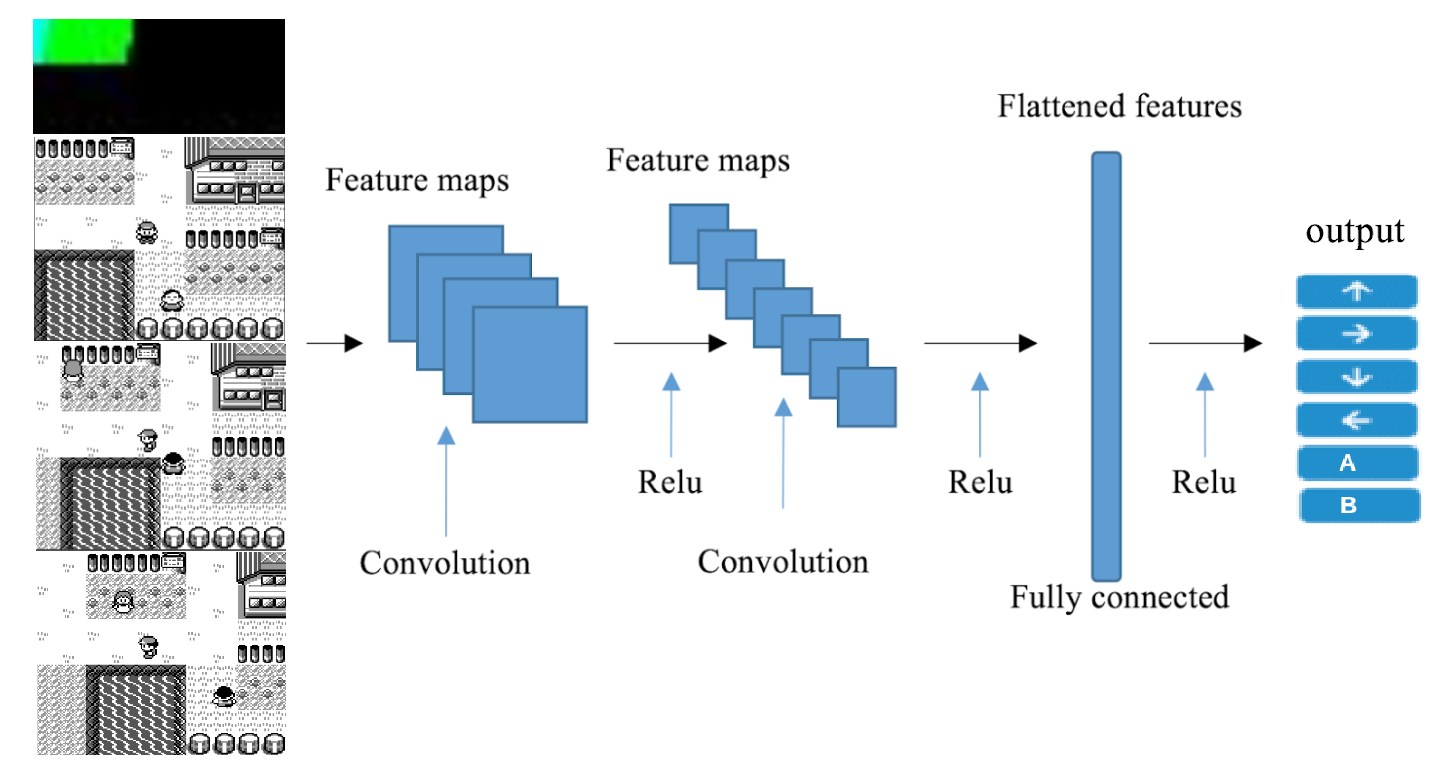
\includegraphics[width=\textwidth]{figs/CNN.png}}
  \caption{The CNN network used for policy and value estimation in the PPO algorithm.}
  \label{fig:cnn}
\end{figure*}



\subsection{Training Procedure}

The training process involves alternating between emulating the game and updating the network. Emulation is performed on the CPU, with one emulator running per core in parallel. Each training step represents some frames being emulated. In each step, the player does an action (a button press and release) from the available actions in his action space, which are: Button A, Button B, Up, Down, Left or Right. 

An episode of the game is a fixed number of steps that is considered as a round of the game. After the episode is over, the game is reset to the initial state and the training continues with the new trained network. 

The rollout buffer stores the game states and rewards of the recent emulation steps and is crucial for training. It is the memory bottleneck of the algorithm, and it's used in the training process to update the network. As the buffer can  easily get large, a batch size equal to 128 is specified in the algorithm. This means that only a subset of 128 states are randomly selected in the buffer at each training stage.

It would be ideal to have an episode length long enough to finish the storyline of the game, and rollout buffers large enough to store all steps from these episodes. This would allow the algorithm to converge in less iterations. However, this type of game has a long gameplay, and thus would require unachievable amounts of memory for the buffer and long processing times for emulating full episodes, which is a CPU-bound task.

To be able to fit the model in memory and train it in reasonable time, the episode length was originally set to 24576 steps, which should be long enough for the player to beat the first gym in the game. The rollout buffer size was set to a value of n\_cpus * episode\_length // 8, being n\_cpus the number of available CPU cores. This configuration means that the model is trained eight times per episode in each CPU, balancing the need for frequent updates with computational resource constraints.





\subsection{Algorithm Configuration}
The same CNN policy from the original work was used \ref{fig:cnn}. It consists of a single network shared between the value and policy functions, and employs a simple convolutional neural network (CNN) architecture inspired by the original Deep Q-Network (DQN) paper by Mnih et al. (2015) \cite{ref:dqn}. This CNN consists of three convolutional layers followed by activation functions (ReLU), a flattening layer, and a single fully connected layer. 

The State input of the network is an image containing the last three frames of the game downscaled and concatenated to a pre-processed health points (HP) bar, facilitating short-term memory and enhancing HP-related rewards. The optimizer used for training is the Adam optimizer with default parameters, excluding weight decay. 

The original proposed network used the following constant hyperparameters:

\begin{itemize}
  \item Learning rate: \(3 \times 10^{-4}\)
  \item Batch size: 128
  \item Entropy coefficient: 0
  \item Weight decay in Adam optimizer: 0
  \item Number of epochs: 3
  \item Gamma: 0.998
\end{itemize}

In this work, I experimented with the first four hyperparameters, varying them to find the best configuration for faster convergence without losing performance. The number of epochs and gamma were kept constant.





\subsection{Reward Calculation}

The same reward calculation proposed originally was used, based on several metrics related to Pokémon gameplay:

\begin{itemize}
  \item Event reward: Rewards for specific in-game events being triggered, such as discovering a new area of the map. This should increase exploration of the map.
  \item Total party level reward: Reward proportional to the cumulative levels of all Pokémon in the player's party. This should motivate the agent to capture new Pokemon and level them up by winning battles.
  \item Healing reward: Rewards for the healing actions performed, proportional to the amount of HP restored. This should motivate the agent to use healing items and to visit Pokemon centers, which is important since they work as checkpoints when the player loses a battle.
  \item Maximum opponent level reward: Rewards for defeating high-level opponents. As the level of the opponents increase throughout the game, this should motivate the agent to follow the storyline.
  \item Gym badges reward: Rewards for earning gym badges. Should motivate the agent to progress through the game.
  \item Exploration reward: The most important reward, based on the number of unique frames the player has explored. It should directly impact the exploration of the map. The algorithm uses a KNN algorithm to compare the current screen's pixels to a list of previously seen screens. If the screen is new, it is added to the list, encouraging the agent to explore new areas of the game.
  \item Dying penalty: Penalties (negative rewards) are applied when the player loses a battle, causing a reset to the last visited Pokémon Center. This is particularly important since the player can be sent far back in the game after losing a battle.
\end{itemize}



\newpage



\section{Experiments and Results}

All experiments were conducted under the following fixed hyperparameters:

\begin{itemize}
  \item Number of CPU cores: 12 (episodes running in parallel).
  \item Total training steps: 68714496, i.e: 233 episodes per CPU.
  \item Episode length: 24576 steps.
  \item Steps per update: 2048, i.e: update model 12 times per episode.
\end{itemize}

Due to the CPU-bound nature of the training algorithm, the training time for all models was approximately the same.  Each model took between 20 and 22 hours to be trained for 233 episodes.

Looking for convergence speed without losing performance, the following models were tried:

\begin{enumerate}
  \item \textbf{Baseline}: The original model with small batch size (128), constant learning rate of \(3 \times 10^{-4}\), no entropy and no weight decay.
  This model did not converge in 68M steps and continued to perform closely to random actions after 68M steps of training, as shown in Fig.\ref{fig:total_reward}.

  \item \textbf{AdamW}: Variation using AdamW optimizer with weight decay equal to \(1 \times 10^{-4}\).
  Performed closely to the baseline model with no notable improvements or deterioration (Fig.\ref{fig:total_reward}).

  \item \textbf{Dynamic Learning Rate}: Dynamic learning rate that decreases logarithmically from \(5 \times 10^{-3}\) to \(5 \times 10^{-5}\);
  Performed closely to the baseline model with no notable improvements or deterioration (Fig.\ref{fig:total_reward}).

  \item \textbf{Large Batch}: Large batch size (50\% of rollout buffer size).
  Performed much better than the others before. Quickly achieved very small loss function values (Figures \ref{fig:entropy_loss}, \ref{fig:value_loss}, \ref{fig:policy_loss}) for both value and policy but got stuck in a local minimum, focusing on training the initial Pokémon without capturing others or visiting Pokemon centers for healing (Fig.\ref{fig:healr}). Of all models, this one demonstrated by far the best map exploration (above 3000 frames), but followed a poor long-term strategy by not capturing new Pokémon. It is the only model that surprisingly learned to not capture any Pokémon, which happened around step 8M (Fig.\ref{fig:pcount}). It got so many rewards from exploring the map that it stopped considering other rewards relevant.

  \item \textbf{Large Batch + Dynamic Learning Rate}: Large batch size (50\% of rollout buffer size) and dynamic learning rate that decreases logarithmically from 5e-3 to 5e-5.
  This model was the most consistent one for this number of steps (68M). It showed the capacity to get total rewards as high as model 4 and learned to heal and capture Pokemon, but explored the map less. Of all models, it got the best healing reward (Fig.\ref{fig:healr}), the best sum of party level reward (Fig.\ref{fig:levels_sum}), and converged the entropy loss function to the smallest value (Fig.\ref{fig:entropy_loss}), but did not learn to explore the map as well as models 4 or 6, staying at around 1000 frames only. The total reward seems to have converged to around 260 (with maxes around 300) but more training would be required to be sure.

  \item \textbf{Large Batch + Entropy}: Large batch size (50\% of rollout buffer size) and entropy coefficient of 0.02.
  Exhibited the most promising results for training longer, showing the highest total rewards and the second highest exploration rate (Fig.\ref{fig:frames}). It learned to heal and capture Pokemon almost as efficiently as model 5, was the only model to pass the 350 total rewards mark (Fig.\ref{fig:total_reward}), and kept a good exploration rate (around 1800 frames). We can infer from the loss functions (Figures \ref{fig:entropy_loss}, \ref{fig:value_loss}, \ref{fig:policy_loss}) that this model would still need more training to converge, however, it already shows similar rewards to model 5 with a much better exploration score. Despite not fully converging, it indicated potential for being the best model among those tested, contingent on further training.

  \item \textbf{Dynamic Learning Rate + Dynamic Batch}: Dynamic learning rate that decreases logarithmically from \(5 \times 10^{-3}\) to \(5 \times 10^{-5}\), and dynamic batch size that increases exponentially from 32 to 6144 (25\% of rollout buffer size).
  Performed particularly worse than all others, converging to a seemingly random and ineffective strategy with small value and policy losses but a relatively large entropy loss, as shown in Figures \ref{fig:entropy_loss}, \ref{fig:value_loss}, \ref{fig:policy_loss}.

\end{enumerate}


\begin{figure}[h]
  \centering
  \fbox{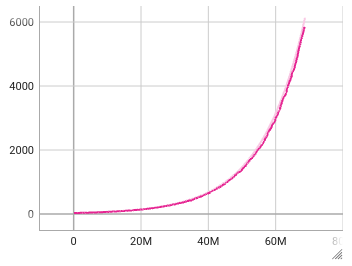
\includegraphics[width=\columnwidth]{exponential.png}}
  \caption{Exponential batch size on model 7.}
  \label{fig:exp}
\end{figure}



\newpage



\section{Conclusions and Future Work}

Throughout this research, I aimed to find a reinforcement learning model that could converge within 20 hours of training while achieving average performance compared to the original setup. The experiments involved various configurations of batch size, learning rate, entropy coefficient, and optimizer types. The baseline model (Model 1) did not converge, performing similarly to random actions even after 68 million steps. Models 2 and 3 showed no notable improvements over the baseline, indicating that neither the AdamW optimizer nor the dynamic learning rate alone provided significant benefits, while Model 7 (Dynamic LR + Dynamic Batch size) performed even worse than the baseline, quickly converging to an ineffective strategy.

Among the models, Model 4 (Large Batch) performed significantly better than the initial configurations by quickly achieving small loss values and demonstrating superior map exploration. However, it fell into a local minimum, focusing solely on training the initial Pokémon without capturing new ones or healing. Model 5 (Large Batch + Dynamic LR) emerged as the most consistent model within the 68 million steps, balancing exploration, healing, and capturing Pokémon effectively, though its map exploration was limited. Model 6 (Large Batch + Entropy) showed the highest potential for further training, achieving the highest total rewards and a good balance between exploration and efficient gameplay. 

These findings suggest that larger batch sizes combined with dynamic learning rates and entropy coefficients, can enhance the training efficiency and performance of reinforcement learning models in complex RPG game environments like Pokémon Red. Further research and extended training could refine these approaches for even better results.

It is important to note that the proposed strategies have not been exhaustively tested. Models may perform better with different parameters, especially those with dynamic learning rates and batch sizes, which could benefit from a deeper study varying minimum and maximum values and using different increasing/decreasing policies, such as linear. Additionally, my tests were limited by the available hardware. A follow-up study using larger batch sizes could be beneficial. For instance, utilizing 100\% of the rollout buffer in the same scenario would require approximately 20 GB of RAM and 12 GB of VRAM. This suggests that with slightly better hardware, the models might achieve even more promising results, highlighting potential areas for future research.



% conference papers do not normally have an appendix


% use section* for acknowledgment
% \section*{Acknowledgment}
% The authors would like to thank...



% trigger a \newpage just before the given reference
% number - used to balance the columns on the last page
% adjust value as needed - may need to be readjusted if
% the document is modified later
%\IEEEtriggeratref{8}
% The "triggered" command can be changed if desired:
%\IEEEtriggercmd{\enlargethispage{-5in}}

% references section

% can use a bibliography generated by BibTeX as a .bbl file
% BibTeX documentation can be easily obtained at:
% http://mirror.ctan.org/biblio/bibtex/contrib/doc/
% The IEEEtran BibTeX style support page is at:
% http://www.michaelshell.org/tex/ieeetran/bibtex/
% \bibliographystyle{IEEEtran}
% argument is your BibTeX string definitions and bibliography database(s)
% \bibliography{example}

% <OR> manually copy in the resultant .bbl file
% set second argument of \begin to the number of references
% (used to reserve space for the reference number labels box)


\begin{thebibliography}{1}

\bibitem{ref:whidden}
Peter Whidden. Playing Pokemon Red with Reinforcement Learning (2023).
Code: \url{https://github.com/PWhiddy/PokemonRedExperiments}.

\bibitem{ref:dqn}
Volodymyr Mnih, Koray Kavukcuoglu, David Silver, Andrei A Rusu, Joel Veness, Marc G Bellemare,
Alex Graves, Martin Riedmiller, Andreas K Fidjeland, Georg Ostrovski, et al. 
Human-level control through deep reinforcement learning. \href{www.nature.com/articles/nature14236}{Nature, 518(7540):529–533} (2015).

\bibitem{ref:ale}
Bellemare, M. G., Naddaf, Y., Veness, J. \& Bowling, M.
The arcade learning environment: An evaluation platform for general agents. \href{https://jair.org/index.php/jair/article/view/10819}{J. Artif. Intell. Res. 47, 253–279} (2013). 

\bibitem{ref:ppo}
John Schulman, Filip Wolski, Prafulla Dhariwal, Alec Radford, Oleg Klimov.
Proximal Policy Optimization Algorithms. \href{https://arxiv.org/abs/1707.06347}{Res arXiv:1707.06347 [cs.LG]} (2017)

\bibitem{ref:dqn2}
Melrose Roderick, James MacGlashan, Stefanie Tellex.
Implementing the Deep Q-Network. \href{https://arxiv.org/abs/1711.07478}{Res arXiv:1711.07478 [cs.LG]} (2017)

\bibitem{ref:stable-baselines3}
\href{https://stable-baselines3.readthedocs.io}{Stable-Baselines3} - Reliable Reinforcement Learning Implementations.

\bibitem{ref:gymnasium}
\href{https://gymnasium.farama.org}{Gymnasium} - An API standard for reinforcement learning with a diverse collection of reference environments.

\end{thebibliography}



% \newpage


\section{Annexes}

% annexes


\begin{figure*}[htbp]
  \centering
  \begin{minipage}[b]{\textwidth}
    \centering
    \fbox{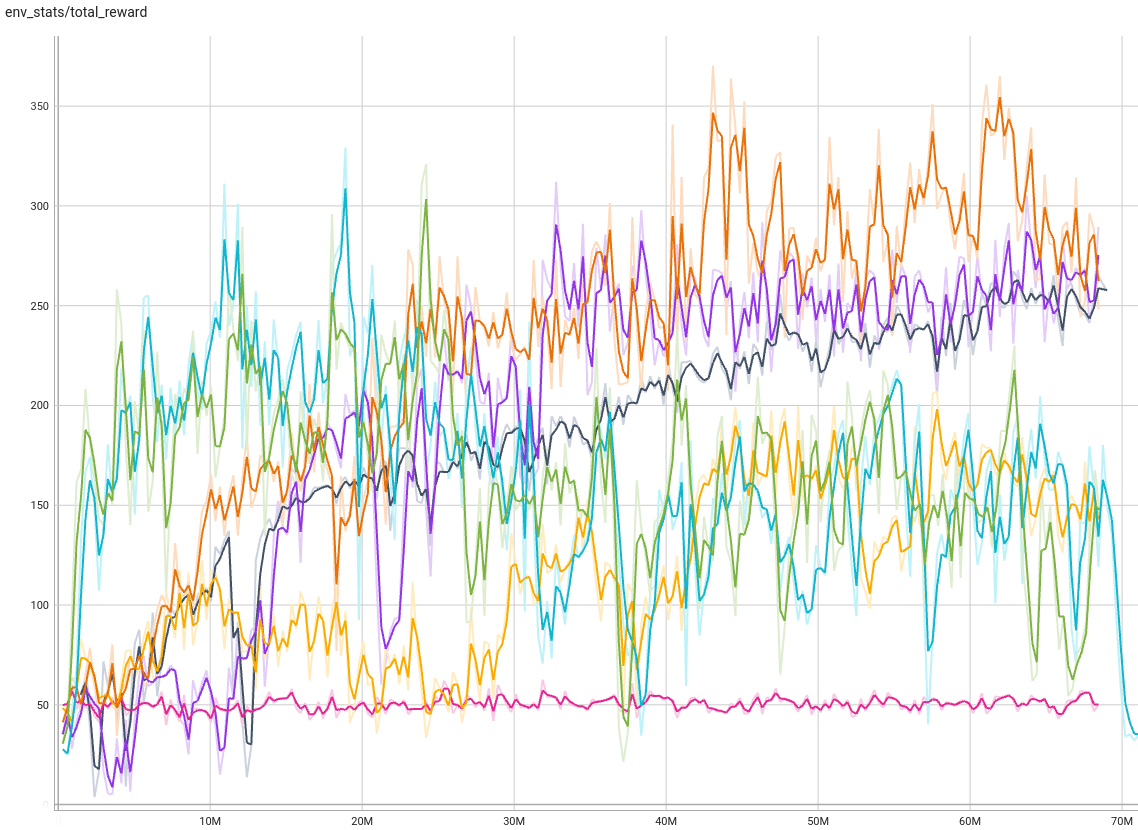
\includegraphics[width=\textwidth]{figs/annex_total_reward.png}}
  \end{minipage}
  \hfill
  \begin{minipage}[b]{\textwidth}
    \centering
    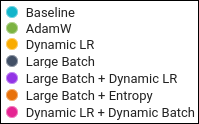
\includegraphics{figs/legend.png}
    \caption{Total reward during training.}
    \label{fig:total_reward}
  \end{minipage}
\end{figure*}

\begin{figure*}[htbp]
  \centering
  \begin{minipage}[b]{\textwidth}
    \centering
    \fbox{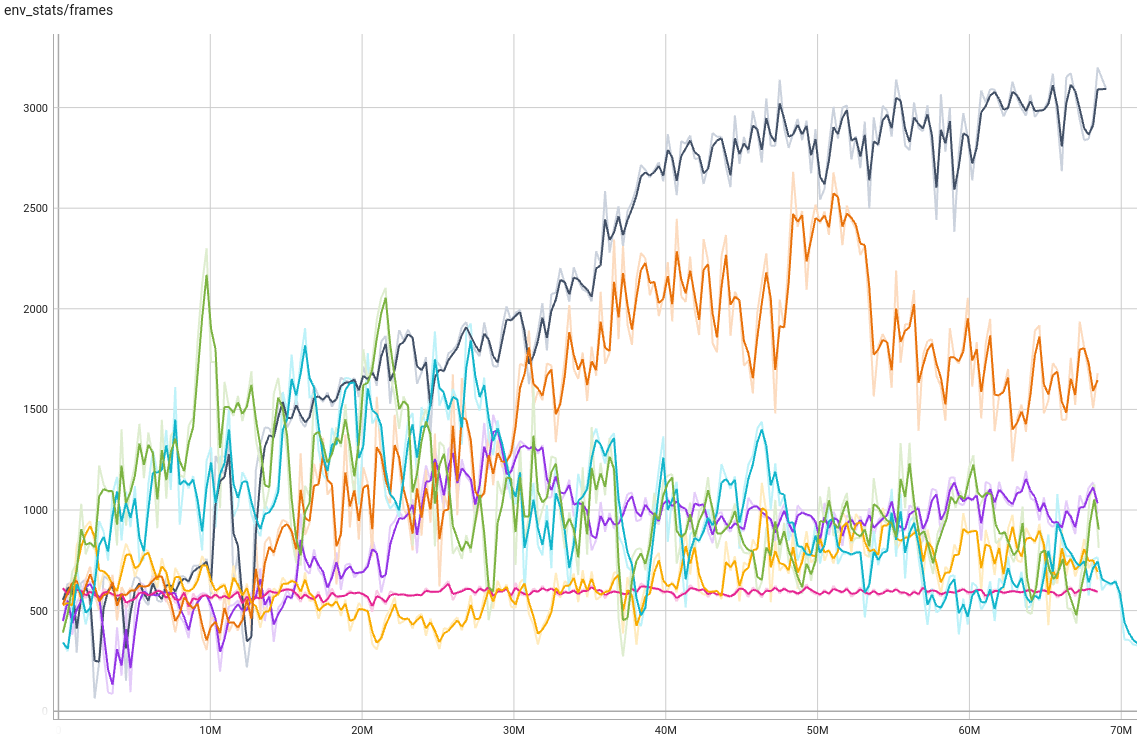
\includegraphics[width=\textwidth]{figs/annex_frames.png}}
  \end{minipage}
  \hfill
  \begin{minipage}[b]{\textwidth}
    \centering
    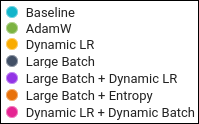
\includegraphics{figs/legend.png}
    \caption{Number of explored frames during training.}
    \label{fig:frames}
  \end{minipage}
\end{figure*}

\begin{figure*}[htbp]
  \centering
  \begin{minipage}[b]{\textwidth}
    \centering
    \fbox{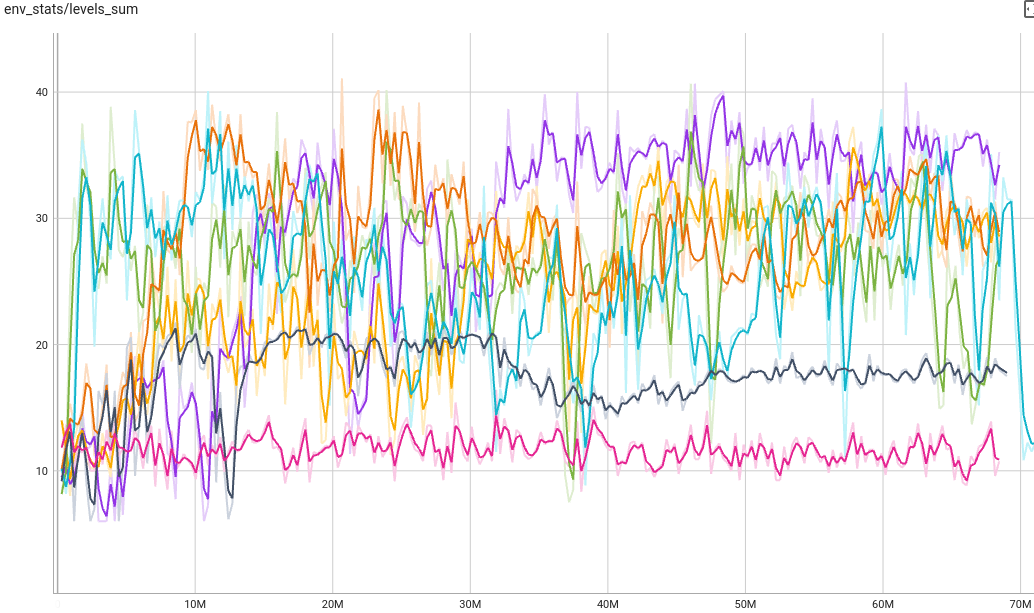
\includegraphics[width=\textwidth]{figs/annex_levels_sum.png}}
  \end{minipage}
  \hfill
  \begin{minipage}[b]{\textwidth}
    \centering
    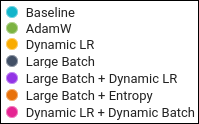
\includegraphics{figs/legend.png}
    \caption{Healing reward during training.}
    \label{fig:levels_sum}
  \end{minipage}
\end{figure*}

\begin{figure*}[htbp]
  \centering
  \begin{minipage}[b]{\textwidth}
    \centering
    \fbox{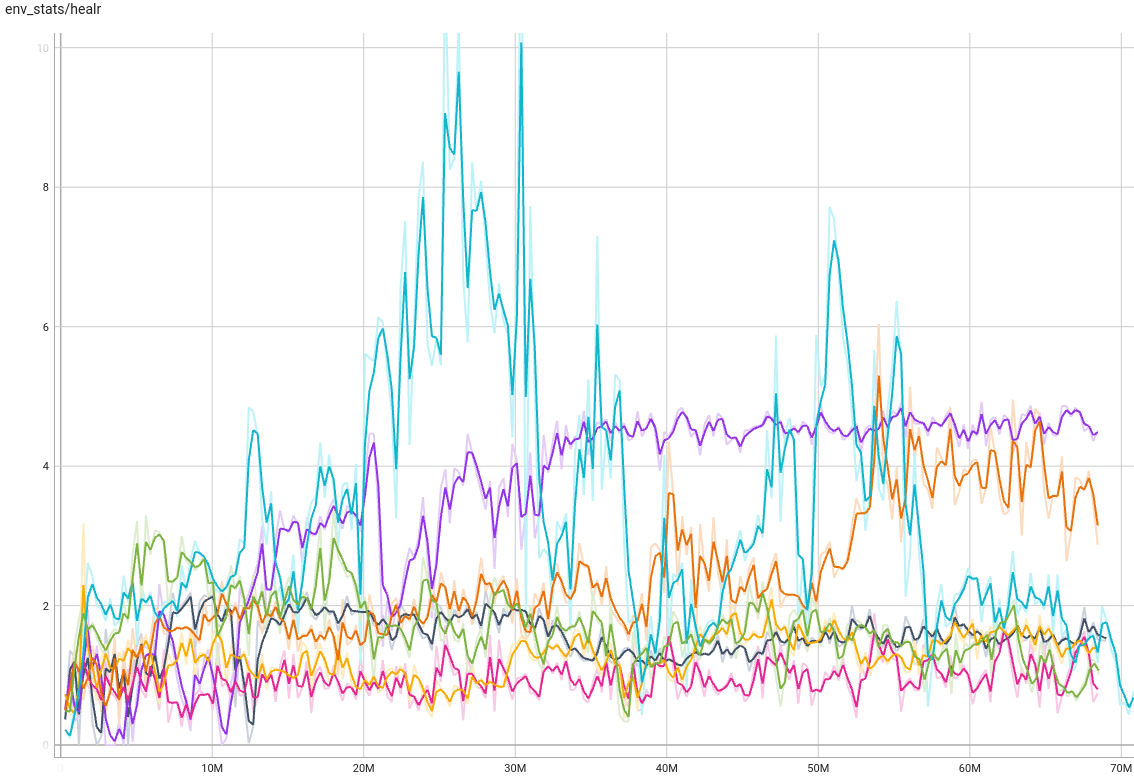
\includegraphics[width=\textwidth]{figs/annex_healr.png}}
  \end{minipage}
  \hfill
  \begin{minipage}[b]{\textwidth}
    \centering
    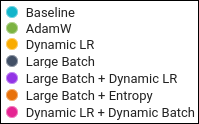
\includegraphics{figs/legend.png}
    \caption{Sum of levels of Pokémon party during training.}
    \label{fig:healr}
  \end{minipage}
\end{figure*}

\begin{figure*}[htbp]
  \centering
  \begin{minipage}[b]{\textwidth}
    \centering
    \fbox{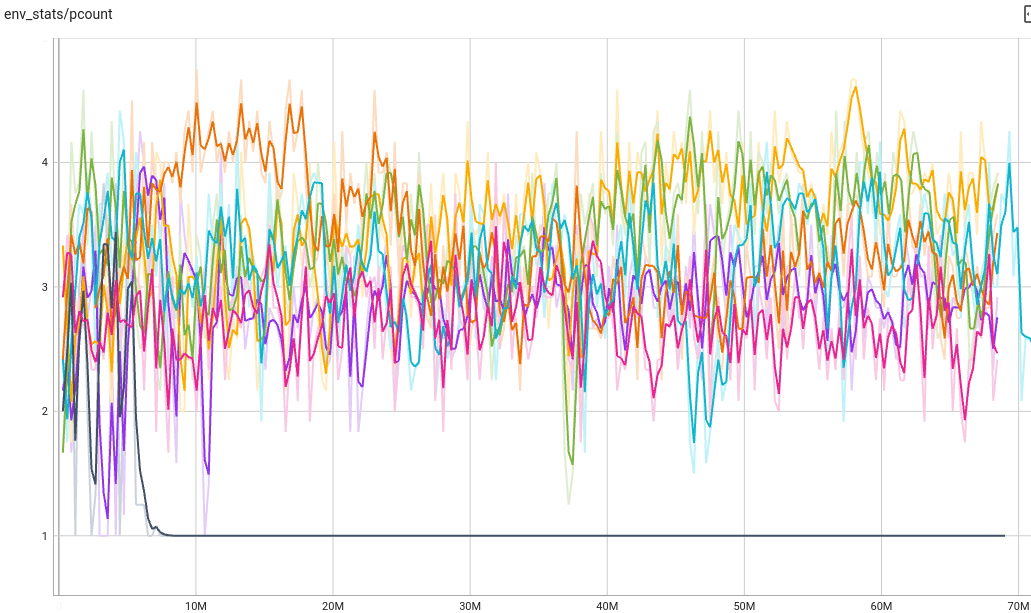
\includegraphics[width=\textwidth]{figs/annex_pcount.png}}
  \end{minipage}
  \hfill
  \begin{minipage}[b]{\textwidth}
    \centering
    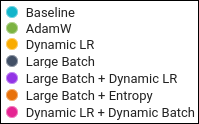
\includegraphics{figs/legend.png}
    \caption{Number of Pokémon in the party during training.}
    \label{fig:pcount}
  \end{minipage}
\end{figure*}

\begin{figure*}[htbp]
  \centering
  \begin{minipage}[b]{\textwidth}
    \centering
    \fbox{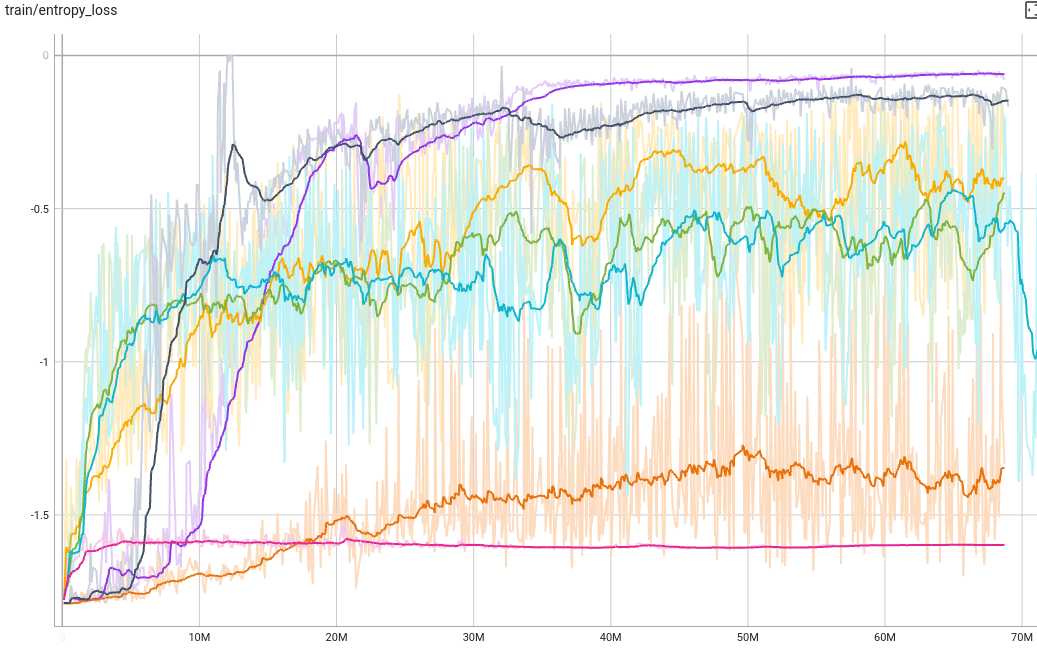
\includegraphics[width=\textwidth]{figs/annex_entropy_loss}}
  \end{minipage}
  \hfill
  \begin{minipage}[b]{\textwidth}
    \centering
    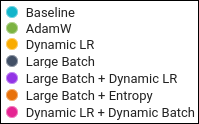
\includegraphics{figs/legend.png}
    \caption{Entropy function loss (smoothed).}
    \label{fig:entropy_loss}
  \end{minipage}
\end{figure*}

\begin{figure*}[htbp]
  \centering
  \begin{minipage}[b]{\textwidth}
    \centering
    \fbox{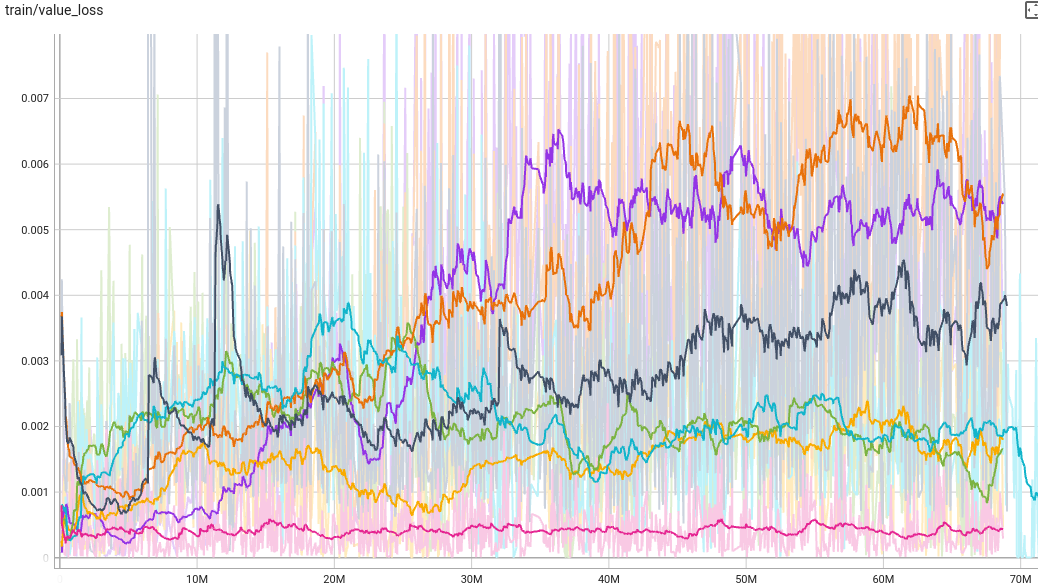
\includegraphics[width=\textwidth]{figs/annex_value_loss}}
  \end{minipage}
  \hfill
  \begin{minipage}[b]{\textwidth}
    \centering
    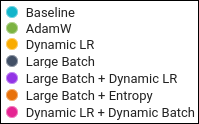
\includegraphics{figs/legend.png}
    \caption{Value function loss (smoothed).}
    \label{fig:value_loss}
  \end{minipage}
\end{figure*}

\begin{figure*}[htbp]
  \centering
  \begin{minipage}[b]{\textwidth}
    \centering
    \fbox{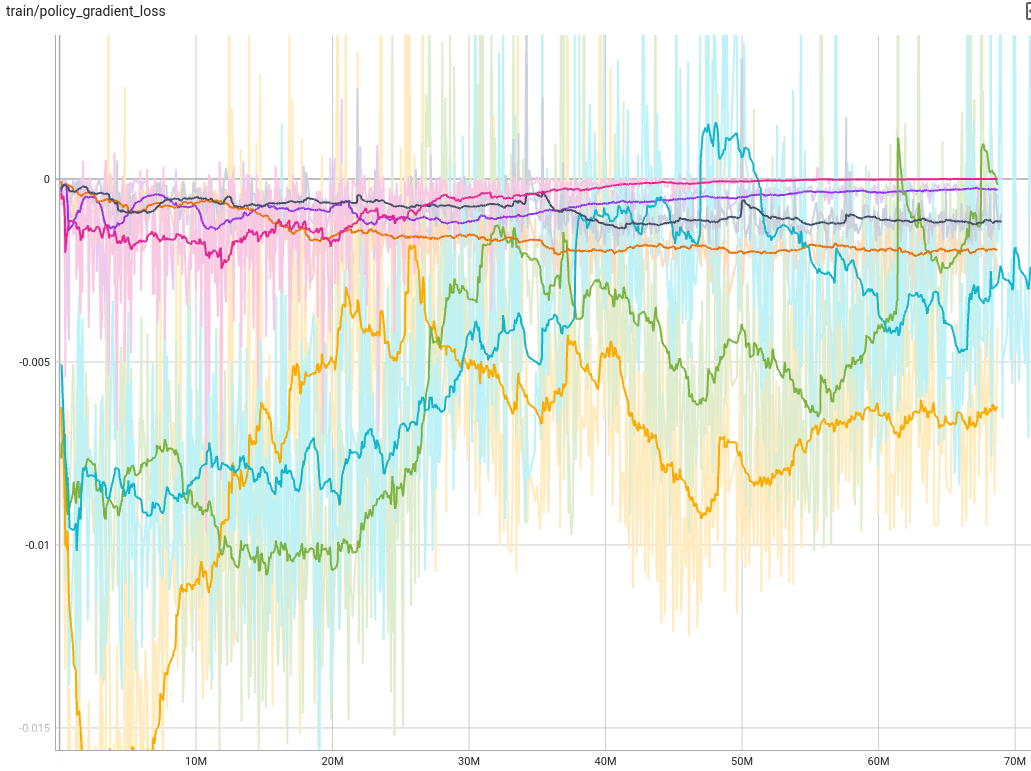
\includegraphics[width=\textwidth]{figs/annex_policy_loss}}
  \end{minipage}
  \hfill
  \begin{minipage}[b]{\textwidth}
    \centering
    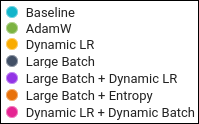
\includegraphics{figs/legend.png}
    \caption{Policy function loss (smoothed).}
    \label{fig:policy_loss}
  \end{minipage}
\end{figure*}



% that's all folks
\end{document}
